\subsection{$\overline{K_n \cup claw \: m}$}
La familia consiste en un grafo $K_n$ y un grafo claw o estrella formado por un nodo y m nodos adyacentes, 
unidos de forma disjunta, que es luego complementado.
\begin{figure}[H]
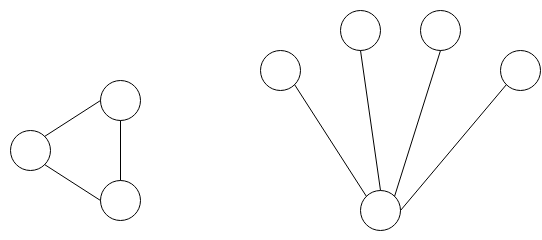
\includegraphics[width=80mm]{K3UC4.png}
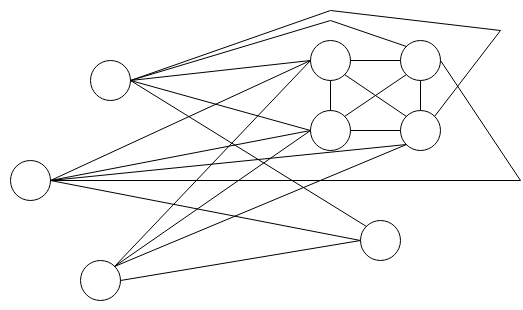
\includegraphics[width=80mm]{K3UC4Complemento.png}
\caption{Ejemplificación: La figura de la izquierda corresponde a $K_3$ $\cup$ $claw$ $4$, 
la figura derecha $\overline{K_3 \cup claw \: 4}$}
\label{overflow}
\end{figure}

\subsection{Grafo Completo $K_n$}
Un grafo completo es un grafo simple donde cada par de vértices está conectado por una arista.
Un grafo completo de n vértices tiene n(n-1)/2 aristas.
Es un grafo regular con todos sus vértices de grado n-1.

\begin{figure}[H]
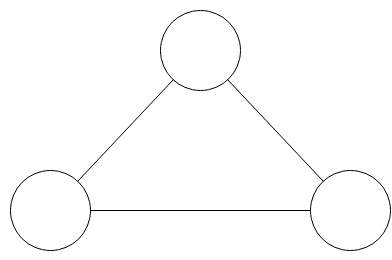
\includegraphics[width=80mm]{K3.png}
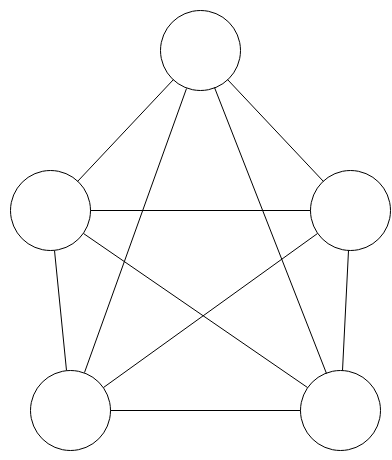
\includegraphics[width=80mm]{K5.png}
\caption{La figura de la izquierda corresponde a un grafo $K_3$ y la figura derecha a un grafo $K_5$.}
\label{overflow}
\end{figure}

\subsection{Grafo Bipartito Completo $K_{n,m}$}
Un grafo bipartito completo es aquel grafo bipartito en el que todos los vértices de la partición $V_1$ están conectados a todos los vértices de la partición $V_2$ y viceversa.

Donde un grafo bipartito es un grafo G=(V,E) cuyos vértices se pueden separar en dos conjuntos disjuntos $V_1$ y $V_2$, es decir, tal que se cumple:
$V_1$ $\cup$ $V_2$ = V
$V_1$ $\cap$ $V_2$ = $\emptyset$
de manera que las aristas sólo pueden conectar vértices de un conjunto con vértices del otro; es decir:
$\forall u_1, u_2 \in V_1, \forall v_1, v_2 \in V_2$ no existe ninguna arista e=($u_1$,$u_2$) ni e=($v_1$,$v_2$).

\begin{figure}[H]
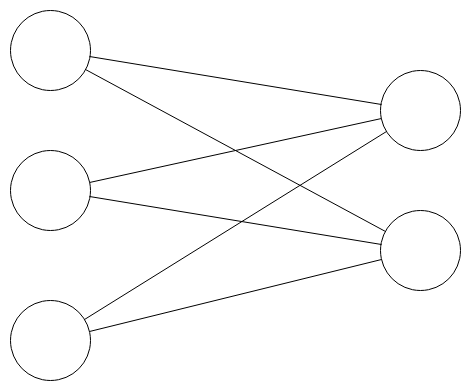
\includegraphics[width=80mm]{K3_2.png}
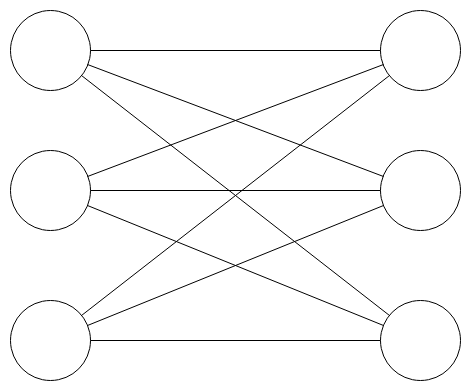
\includegraphics[width=80mm]{K3_3.png}
\caption{La figura de la izquierda corresponde a un grafo bipartito completo $K_{3,2}$ y la figura derecha a un grafo bipartito completo $K_{3,3}$.}
\label{overflow}
\end{figure}


\subsection{Grafo Lattice $L_{m,n}$}
Un grafo Lattice es el producto cartesiano de dos grafos completos $K_m$ y $K_n$.

\begin{figure}[H]
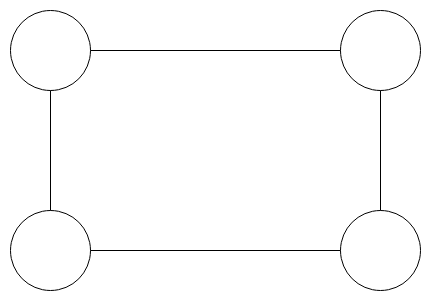
\includegraphics[width=80mm]{L2_2.png}
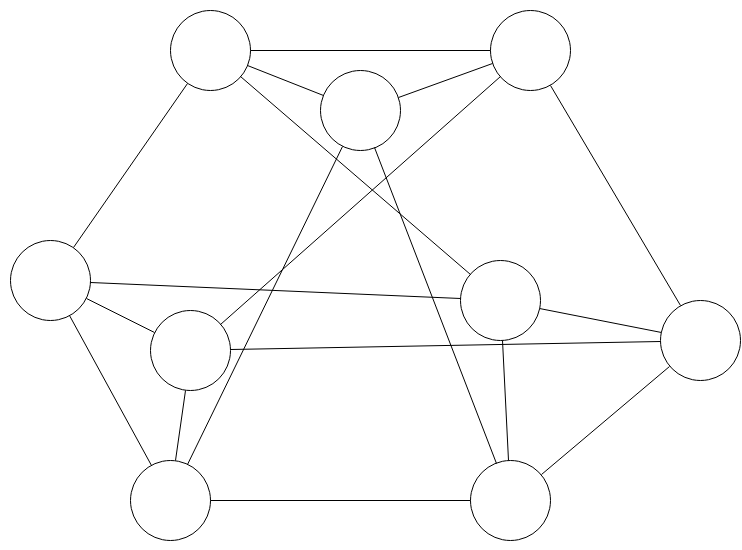
\includegraphics[width=80mm]{L3_3.png}
\caption{La figura de la izquierda corresponde a un grafo Lattice $L_{2,2}$ y la figura derecha a un grafo Lattice $L_{3,2}$.}
\label{overflow}
\end{figure}

\subsection{Grafo Claw}
Un grafo claw es un grafo bipartito completo $K_{1,n}$. Un único vértice que se une con n vértices y entre los n vértices no existen aristas.

\begin{figure}[H]
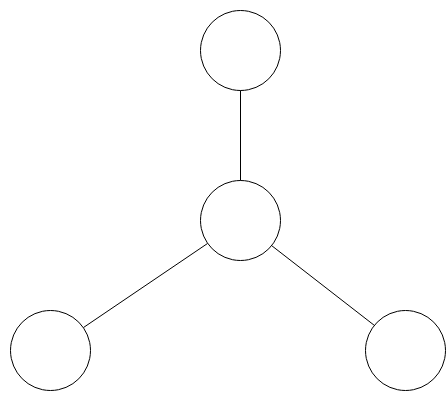
\includegraphics[width=80mm]{K1_3.png}
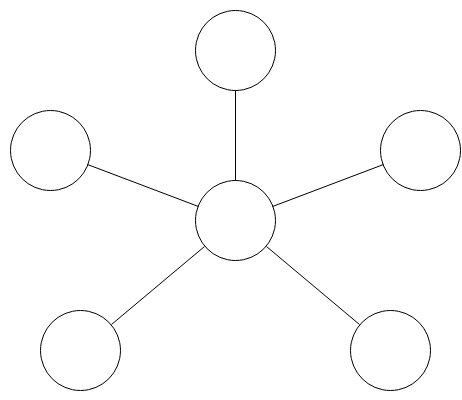
\includegraphics[width=80mm]{K1_5.png}
\caption{La figura de la izquierda corresponde a un grafo claw $K_{1,3}$ y la figura derecha a un grafo claw $K_{1,5}$.}
\label{overflow}
\end{figure}

\subsection{Grafo Path $P_n$}
Un grafo path es un grafo es una sucesión de aristas $e_1e_2$...$e_k$ tal que un extremo de $e_i$ coincide con uno de $e_{i-1}$ y el otro con el de $e_{i+1}$ para i = 2...k-1.

\begin{figure}[H]
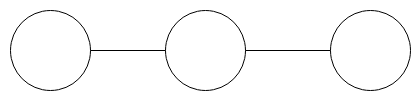
\includegraphics[width=80mm]{P3.png}
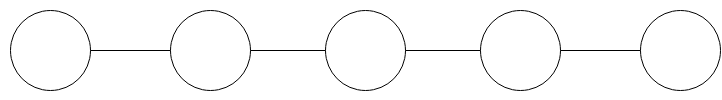
\includegraphics[width=80mm]{P5.png}
\caption{La figura de la izquierda corresponde a un grafo path $P_3$ y la figura derecha a un grafo path $P_5$.}
\label{overflow}
\end{figure}

\subsection{Grafo Fan $F_{m,n}$}
Un grafo fan $F_{m,n}$ se define como la unión de $\overline{K}_m$ y $P_n$.

Donde $\overline{K}_m$ es un grafo con $m$ nodos y 0 aristas y $P_n$ es un grafo path.

\begin{figure}[H]
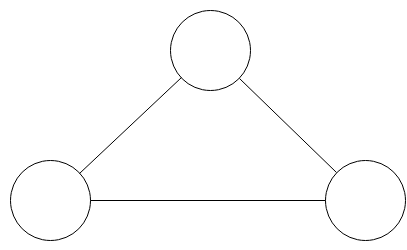
\includegraphics[width=80mm]{F1_2.png}
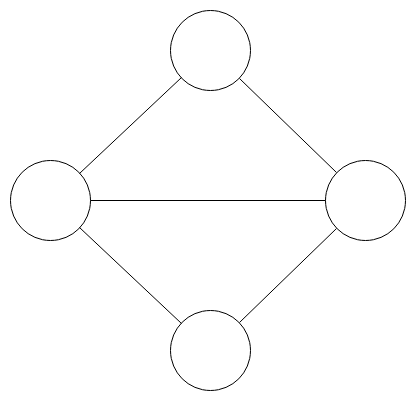
\includegraphics[width=80mm]{F1_3.png}
\caption{La figura de la izquierda corresponde a un grafo fan $F_{1,2}$ y la figura derecha a un grafo fan $F_{1,3}$.}
\label{overflow}
\end{figure}

\subsection{Grafo cicle $C_n$}
Un Grafo cicle $C_n$, es un grafo que se asemeja a un polígono de n lados. Consiste en un camino cerrado en el que no se repite ningún vértice a excepción del primero que aparece dos veces como principio y fin del camino. 

\begin{figure}[H]
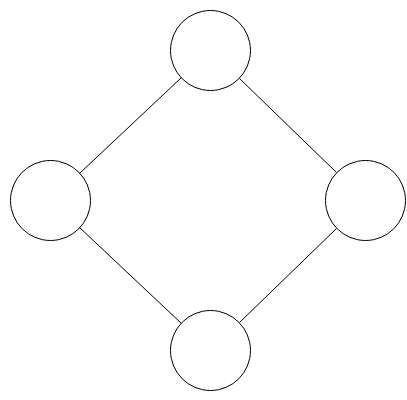
\includegraphics[width=80mm]{C_4.png}
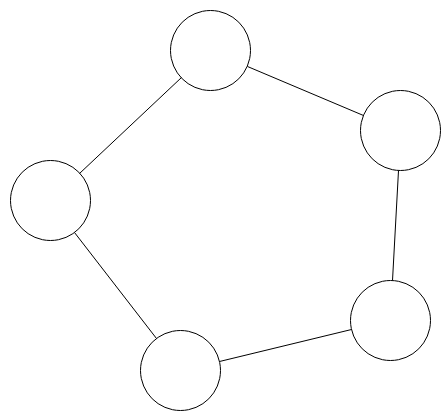
\includegraphics[width=80mm]{C_5.png}
\caption{La figura de la izquierda corresponde a un grafo cicle $C_4$ y la figura derecha a un grafo cicle $C_5$.}
\label{overflow}
\end{figure}
